\documentclass[11pt, a4paper]{article}

% ----- Packages -----
\usepackage[utf8]{inputenc}
\usepackage{amsmath, amssymb, amsthm, mathtools}
\usepackage{geometry}
\geometry{top=1in, bottom=1in, left=0.9in, right=0.9in}
\usepackage{float}
\usepackage{tikz}
\usepackage{booktabs}
\usepackage{graphicx}
\usepackage{fancyhdr}
\usepackage{lastpage}
\usepackage[colorlinks=true, linkcolor=black, citecolor=black, urlcolor=black]{hyperref}
\usepackage[capitalise, noabbrev]{cleveref}
\usetikzlibrary{arrows.meta, positioning, patterns, calc}
\usepackage{pgfplots}
\usepackage{pgfplotstable}
\pgfplotsset{compat=1.18}
\usepgfplotslibrary{fillbetween}

% ----- Fancy Headers/Footers -----
\pagestyle{fancy}
\fancyhf{}
\fancyhead[L]{\small CE 512 --- Finite Element Method}
\fancyhead[R]{\small Homework 2}
\fancyfoot[C]{\small Page \thepage\ of \pageref{LastPage}}
\renewcommand{\headrulewidth}{0.4pt}
\renewcommand{\footrulewidth}{0.4pt}

% ----- TikZ Styles -----
\tikzset{
    feNode/.style={circle, draw=black, fill=white, thick, inner sep=0pt, minimum size=1.8mm},
    nodeLabel/.style={circle, draw=black, fill=white, inner sep=1pt, font=\footnotesize\bfseries, minimum size=5mm},
    elemLabel/.style={rectangle, draw=black, fill=white, inner sep=2pt, font=\footnotesize\bfseries, minimum size=4mm},
    dimLine/.style={{Latex[length=2.5mm, width=1.5mm]}-{Latex[length=2.5mm, width=1.5mm]}, thin},
    extLine/.style={thin, draw=black!70},
    feLine/.style={line width=1.5pt}
}

\begin{document}

% ----- Title Page -----
\begin{titlepage}
\thispagestyle{empty}
\begin{center}
    \vspace*{1cm}
    
\includegraphics[width=0.45\textwidth]{../HW1/iyte_logo eng.pdf}\\[1.5cm]
    {\LARGE \textbf{Homework 2 --- Solutions}}\\[0.8cm]
    {\Large \textbf{CE 512 Finite Element Method}}\\[0.4cm]
    {\Large 2026 Spring}\\[2.5cm]
    {\large \textbf{Muhammet Ya\u{g}c\i o\u{g}lu}}\\[0.3cm]
    {\large Student No: 290204042}\\[2cm]
    {\large March 4, 2026}
    \vfill
    {\normalsize \textit{\.{I}zmir Institute of Technology}\\Department of Civil Engineering}
\end{center}
\end{titlepage}

% ----- TOC -----
\tableofcontents
\newpage

% ======================================================================
\section{Problem Statement}
% ======================================================================

The four-element plane truss in \cref{fig:problem} has $E=20\,000$~MPa and $\sigma_y=300$~MPa.  All members are made from a square hollow section with outer dimensions $40\times40$~mm and thickness $t=2.5$~mm, so
\[
A = 40^2-35^2 = 375\;\text{mm}^2.
\]
Nodes 1 and 2 are pinned; force $P$ acts downward at node~4.

\begin{figure}[H]
    \centering
    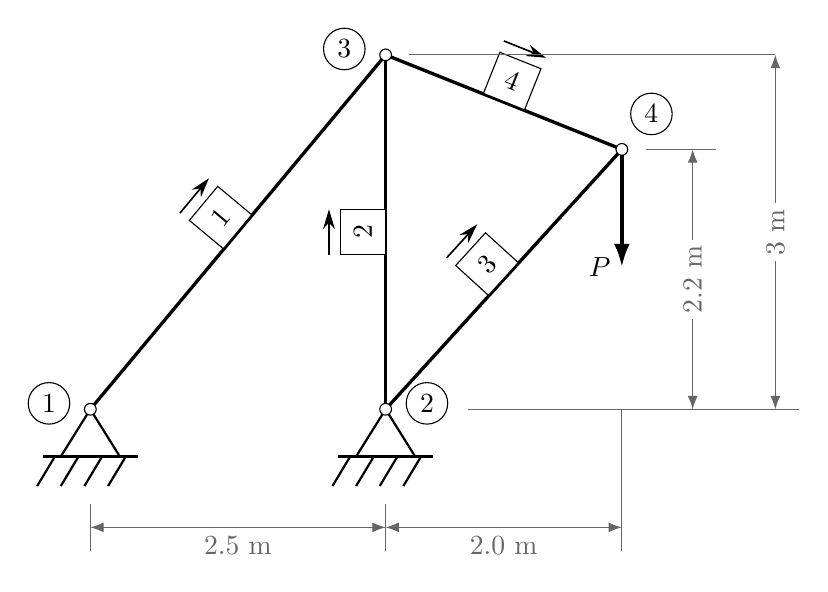
\begin{tikzpicture}[scale=1.5, >={Latex[length=3mm, width=2mm]}]
        
        % Styles
        \tikzset{
            feLine/.style={very thick},
            feNode/.style={circle, draw, fill=white, inner sep=1.5pt, minimum size=4pt},
            nodeLabel/.style={circle, draw, inner sep=1pt, minimum size=15pt},
            extLine/.style={thin, black!60},
            dimLine/.style={<->, >=Latex, thin, black!60}
        }

        % --- Custom Macro for Element Labels ---
        % #1 = Start Node, #2 = End Node, #3 = Element Number
        \newcommand{\drawElement}[3]{
            % Draw the element line
            \draw[feLine] (#1) -- (#2);
            
            % Draw the rectangular box sitting ON the line (anchor=south)
            \path (#1) -- (#2) node[midway, sloped, anchor=south, draw, fill=white, inner sep=2pt, minimum size=16pt] (E#3) {#3};
            
            % Calculate coordinates for the arrow slightly above the box
            % !1.25! means it hovers exactly 25% of the box height above the box itself
            \coordinate (TopLeft#3) at ($(E#3.south west)!1.25!(E#3.north west)$);
            \coordinate (TopRight#3) at ($(E#3.south east)!1.25!(E#3.north east)$);
            
            % Draw the arrow, technical style (Stealth tip, exact width of the box)
            \draw[-{Stealth[length=2.5mm, width=1.5mm]}, semithick] (TopLeft#3) -- (TopRight#3);
        }

        % Coordinates
        \coordinate (N1) at (0, 0);
        \coordinate (N2) at (2.5, 0);
        \coordinate (N3) at (2.5, 3.0);
        \coordinate (N4) at (4.5, 2.2);
        
        % Draw Elements using the custom macro
        \drawElement{N1}{N3}{1}
        \drawElement{N2}{N3}{2}
        \drawElement{N2}{N4}{3}
        \drawElement{N3}{N4}{4}
        
        % Pinned Support Macro
        \def\drawPinSupport#1{
            \draw[thick] (#1) -- ++(-0.25, -0.4) -- ++(0.5, 0) -- cycle;
            \draw[thick] (#1) ++(-0.4, -0.4) -- ++(0.8, 0);
            \foreach \i in {-0.3, -0.1, 0.1, 0.3} {
                \draw[thick] (#1) ++(\i, -0.4) -- ++(-0.15, -0.25);
            }
        }
        
        % Draw Supports
        \drawPinSupport{N1}
        \drawPinSupport{N2}
        
        % Applied Force P
        \draw[->, line width=1.5pt] (N4) -- ++(0, -1.0) node[pos=1, left] {$P$};
        
        % Draw Nodes (circles at joints)
        \node[feNode] at (N1) {};
        \node[feNode] at (N2) {};
        \node[feNode] at (N3) {};
        \node[feNode] at (N4) {};
        
        % Node Labels (circled numbers)
        \node[nodeLabel] at ($(N1)+(-0.35, 0.05)$) {1};
        \node[nodeLabel] at ($(N2)+(0.35, 0.05)$)  {2};
        \node[nodeLabel] at ($(N3)+(-0.35, 0.05)$) {3};
        \node[nodeLabel] at ($(N4)+(0.25, 0.3)$)  {4};
        
        % Dimensioning
        \draw[extLine] (N1) ++(0, -0.8) -- ++(0, -0.4);
        \draw[extLine] (N2) ++(0, -0.8) -- ++(0, -0.4);
        \draw[extLine] (N4) ++(0, -2.2) -- ++(0, -1.2);
        \draw[dimLine] (0, -1.0) -- (2.5, -1.0) node[midway, below] {$2.5$ m};
        \draw[dimLine] (2.5, -1.0) -- (4.5, -1.0) node[midway, below] {$2.0$ m};
        
        \draw[extLine] (3.2, 0) -- (6.0, 0);
        \draw[extLine] (N4) ++(0.2, 0) -- ++(0.6, 0);
        \draw[extLine] (N3) ++(0.2, 0) -- ++(3.1, 0);
        \draw[dimLine] (5.1, 0) -- (5.1, 2.2) node[midway, fill=white, inner sep=2pt, rotate=90] {$2.2$ m};
        \draw[dimLine] (5.8, 0) -- (5.8, 3.0) node[midway, fill=white, inner sep=2pt, rotate=90] {$3$ m};
        
    \end{tikzpicture}
    \caption{Four-element truss structure.}
    \label{fig:problem}
\end{figure}

\noindent\textbf{Required:}\; (a)~Global stiffness matrix.\; (b)~Nodal displacements.\; (c)~Element strains.\; (d)~$P$ at first yield.\; (e)~$P$ at first buckling.

% ======================================================================
\section{Element Connectivity and DOFs}\label{sec:dof}
% ======================================================================

Each node carries DOFs $(u_n,v_n)$; the global DOF vector is $\mathbf{d}=\{u_1,v_1,u_2,v_2,u_3,v_3,u_4,v_4\}^T$.

\begin{figure}[H]
\centering
    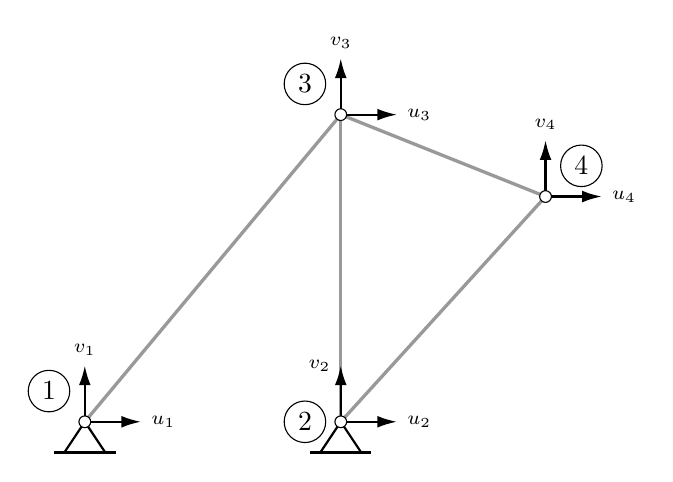
\begin{tikzpicture}[scale=1.3, >={Latex[length=2.5mm, width=1.5mm]}]
        
        % Styles (included so it compiles standalone)
        \tikzset{
            feLine/.style={very thick},
            feNode/.style={circle, draw, fill=white, inner sep=1.5pt, minimum size=4pt},
            nodeLabel/.style={circle, draw, inner sep=1pt, minimum size=15pt}
        }
        
        % Coordinates
        \coordinate (N1) at (0,0);
        \coordinate (N2) at (2.5,0);
        \coordinate (N3) at (2.5,3.0);
        \coordinate (N4) at (4.5,2.2);
        
        % 1. Draw structural lines (bottom-most layer)
        \draw[feLine, black!40] (N1)--(N3);
        \draw[feLine, black!40] (N2)--(N3);
        \draw[feLine, black!40] (N2)--(N4);
        \draw[feLine, black!40] (N3)--(N4);
        
        % 2. Draw supports
        % (Drawn before nodes so the triangle tips don't cover the white circles)
        \draw[thick] (N1) -- ++(-0.2,-0.3) -- ++(0.4,0) -- cycle;
        \draw[thick] ($(N1)+(-0.3,-0.3)$) -- ++(0.6,0);
        \draw[thick] (N2) -- ++(-0.2,-0.3) -- ++(0.4,0) -- cycle;
        \draw[thick] ($(N2)+(-0.3,-0.3)$) -- ++(0.6,0);

        % 3. Draw DOF vectors
        % (Drawn before nodes so the arrow shafts don't cross the white circles)
        \draw[->, thick] (N1) -- ++(0.55,0) node[right, font=\scriptsize]{$u_1$};
        \draw[->, thick] (N1) -- ++(0,0.55) node[above, font=\scriptsize]{$v_1$};
        \draw[->, thick] (N2) -- ++(0.55,0) node[right, font=\scriptsize]{$u_2$};
        \draw[->, thick] (N2) -- ++(0,0.55) node[left, font=\scriptsize]{$v_2$};
        \draw[->, thick] (N3) -- ++(0.55,0) node[right, font=\scriptsize]{$u_3$};
        \draw[->, thick] (N3) -- ++(0,0.55) node[above, font=\scriptsize]{$v_3$};
        \draw[->, thick] (N4) -- ++(0.55,0) node[right, font=\scriptsize]{$u_4$};
        \draw[->, thick] (N4) -- ++(0,0.55) node[above, font=\scriptsize]{$v_4$};
        
        % 4. Draw Nodes (Top layer - covers everything beneath them)
        \foreach \n in {N1,N2,N3,N4} { \node[feNode] at (\n) {}; }
        
        % 5. Draw Node Labels
        \node[nodeLabel] at ($(N1)+(-0.35, 0.3)$) {1};
        \node[nodeLabel] at ($(N2)+(-0.35, 0.0)$)  {2};
        \node[nodeLabel] at ($(N3)+(-0.35, 0.3)$) {3};
        \node[nodeLabel] at ($(N4)+(0.35, 0.3)$)  {4};
        
    \end{tikzpicture}
\caption{Global DOFs.}
\label{fig:dofs}
\end{figure}

\noindent Element connectivity and DOF mapping:
\[
\begin{array}{c|cc|l}
e & i & j & \text{Global DOFs: } (u_i,\,v_i,\,u_j,\,v_j) \\
\hline
1 & 1 & 3 & (u_1,\,v_1,\,u_3,\,v_3) \\
2 & 2 & 3 & (u_2,\,v_2,\,u_3,\,v_3) \\
3 & 2 & 4 & (u_2,\,v_2,\,u_4,\,v_4) \\
4 & 3 & 4 & (u_3,\,v_3,\,u_4,\,v_4) \\
\end{array}
\]

% ======================================================================
\section{Element Geometry}\label{sec:geometry}
% ======================================================================

For element $e$ from node $i\,(x_i,y_i)$ to node $j\,(x_j,y_j)$:
\[
L_e = \sqrt{(\Delta x_e)^2+(\Delta y_e)^2},\qquad
c_e = \frac{\Delta x_e}{L_e},\qquad
s_e = \frac{\Delta y_e}{L_e}.
\]

\begingroup\small
\[
\begin{array}{c|rr|c|cc|ccc|c}
e & \Delta x_e & \Delta y_e & L_e\;\text{(mm)} & c_e & s_e & c_e^2 & s_e^2 & c_e s_e & EA/L_e\\
\hline
1 & 2500 & 3000 & 500\sqrt{61}\approx3905 & \tfrac{5}{\sqrt{61}} & \tfrac{6}{\sqrt{61}} & \tfrac{25}{61} & \tfrac{36}{61} & \tfrac{30}{61} & 1920.55 \\[4pt]
2 & 0 & 3000 & 3000 & 0 & 1 & 0 & 1 & 0 & 2500.00 \\[4pt]
3 & 2000 & 2200 & 200\sqrt{221}\approx2973 & \tfrac{10}{\sqrt{221}} & \tfrac{11}{\sqrt{221}} & \tfrac{100}{221} & \tfrac{121}{221} & \tfrac{110}{221} & 2522.52 \\[4pt]
4 & 2000 & -800 & 400\sqrt{29}\approx2154 & \tfrac{5}{\sqrt{29}} & \tfrac{-2}{\sqrt{29}} & \tfrac{25}{29} & \tfrac{4}{29} & \tfrac{-10}{29} & 3481.79
\end{array}
\]
\endgroup

All $\Delta x$, $\Delta y$ in mm; $EA/L_e$ in N/mm.

% ======================================================================
\section{Part (a): Global Stiffness Matrix}\label{sec:parta}
% ======================================================================

The local stiffness matrix for a truss element is
\begin{equation}
\mathbf{k}^{(e)}_{\text{local}} = \frac{EA}{L_e}
\begin{bmatrix} 1 & -1 \\ -1 & 1 \end{bmatrix}.
\end{equation}

The transformation matrix $\mathbf{T}_e$ relating local DOFs $\{u'_i,\,u'_j\}^T$ to global DOFs $\{u_i, v_i, u_j, v_j\}^T$:
\begin{equation}
\mathbf{T}_e =
\begin{bmatrix} c_e & s_e & 0 & 0 \\ 0 & 0 & c_e & s_e \end{bmatrix}.
\end{equation}

The element stiffness in global coordinates $\mathbf{K}^{(e)}=\mathbf{T}_e^T\,\mathbf{k}^{(e)}_{\text{local}}\,\mathbf{T}_e$ gives
\begin{equation}\label{eq:Ke}
\mathbf{K}^{(e)} = \frac{EA}{L_e}
\begin{bmatrix}
 c_e^2   &  c_e s_e & -c_e^2   & -c_e s_e \\
 c_e s_e &  s_e^2   & -c_e s_e & -s_e^2   \\
-c_e^2   & -c_e s_e &  c_e^2   &  c_e s_e \\
-c_e s_e & -s_e^2   &  c_e s_e &  s_e^2
\end{bmatrix}.
\end{equation}

\noindent\textbf{Element 1} ($1\!\to\!3$, DOFs: $u_1,v_1,u_3,v_3$):

\begingroup\small
\setlength{\arraycolsep}{3pt}
\[
\mathbf{K}^{(1)} = \frac{EA}{L_1}
\begin{bmatrix}
c_1^2 & c_1 s_1 & -c_1^2 & -c_1 s_1 \\
c_1 s_1 & s_1^2 & -c_1 s_1 & -s_1^2 \\
-c_1^2 & -c_1 s_1 & c_1^2 & c_1 s_1 \\
-c_1 s_1 & -s_1^2 & c_1 s_1 & s_1^2
\end{bmatrix}
=
\begin{bmatrix}
 787.11 &   944.53 & -787.11 &  -944.53 \\
 944.53 &  1133.44 & -944.53 & -1133.44 \\
-787.11 &  -944.53 &  787.11 &   944.53 \\
-944.53 & -1133.44 &  944.53 &  1133.44
\end{bmatrix}\;\text{N/mm}
\]
\endgroup

\noindent\textbf{Element 2} ($2\!\to\!3$, DOFs: $u_2,v_2,u_3,v_3$),\; $c_2=0$, $s_2=1$:

\[
\mathbf{K}^{(2)} = 2500
\begin{bmatrix}
0 & 0 & 0 & 0 \\
0 & 1 & 0 & -1 \\
0 & 0 & 0 & 0 \\
0 & -1& 0 & 1
\end{bmatrix}
=
\begin{bmatrix}
0 & 0 & 0 & 0 \\
0 & 2500.00 & 0 & -2500.00 \\
0 & 0 & 0 & 0 \\
0 & -2500.00 & 0 & 2500.00
\end{bmatrix}\;\text{N/mm}
\]

\noindent\textbf{Element 3} ($2\!\to\!4$, DOFs: $u_2,v_2,u_4,v_4$):

\begingroup\small
\setlength{\arraycolsep}{3pt}
\[
\mathbf{K}^{(3)} = \frac{EA}{L_3}
\begin{bmatrix}
c_3^2 & c_3 s_3 & -c_3^2 & -c_3 s_3 \\
c_3 s_3 & s_3^2 & -c_3 s_3 & -s_3^2 \\
-c_3^2 & -c_3 s_3 & c_3^2 & c_3 s_3 \\
-c_3 s_3 & -s_3^2 & c_3 s_3 & s_3^2
\end{bmatrix}
=
\begin{bmatrix}
 1141.41 &  1255.55 & -1141.41 & -1255.55 \\
 1255.55 &  1381.11 & -1255.55 & -1381.11 \\
-1141.41 & -1255.55 &  1141.41 &  1255.55 \\
-1255.55 & -1381.11 &  1255.55 &  1381.11
\end{bmatrix}\;\text{N/mm}
\]
\endgroup

\noindent\textbf{Element 4} ($3\!\to\!4$, DOFs: $u_3,v_3,u_4,v_4$):

\begingroup\small
\setlength{\arraycolsep}{3pt}
\[
\mathbf{K}^{(4)} = \frac{EA}{L_4}
\begin{bmatrix}
c_4^2 & c_4 s_4 & -c_4^2 & -c_4 s_4 \\
c_4 s_4 & s_4^2 & -c_4 s_4 & -s_4^2 \\
-c_4^2 & -c_4 s_4 & c_4^2 & c_4 s_4 \\
-c_4 s_4 & -s_4^2 & c_4 s_4 & s_4^2
\end{bmatrix}
=
\begin{bmatrix}
 3001.54 & -1200.62 & -3001.54 &  1200.62 \\
-1200.62 &   480.25 &  1200.62 &  -480.25 \\
-3001.54 &  1200.62 &  3001.54 & -1200.62 \\
 1200.62 &  -480.25 & -1200.62 &   480.25
\end{bmatrix}\;\text{N/mm}
\]
\endgroup

\noindent Assembling $\mathbf{K}=\sum_{e=1}^{4}\mathbf{A}_e^T\mathbf{K}^{(e)}\mathbf{A}_e$ by the direct stiffness method. The assembled global stiffness matrix is:

\begingroup\small
\setlength{\arraycolsep}{3pt}
\begin{equation}\label{eq:Kglobal}
\mathbf{K} =
\left[\begin{array}{rrrrrrrr}
u_1 & v_1 & u_2 & v_2 & u_3 & v_3 & u_4 & v_4 \\[2pt]
  787.11 &  944.53 &    0    &    0    & -787.11 & -944.53 &    0    &    0    \\
  944.53 & 1133.44 &    0    &    0    & -944.53 &-1133.44 &    0    &    0    \\
    0    &    0    & 1141.41 & 1255.55 &    0    &    0    &-1141.41 &-1255.55 \\
    0    &    0    & 1255.55 & 3881.11 &    0    &-2500.00 &-1255.55 &-1381.11 \\
 -787.11 & -944.53 &    0    &    0    & 3788.65 & -256.08 &-3001.54 & 1200.62 \\
 -944.53 &-1133.44 &    0    &-2500.00 & -256.08 & 4113.69 & 1200.62 & -480.25 \\
    0    &    0    &-1141.41 &-1255.55 &-3001.54 & 1200.62 & 4142.95 &   54.94 \\
    0    &    0    &-1255.55 &-1381.11 & 1200.62 & -480.25 &   54.94 & 1861.36
\end{array}\right]\;\text{N/mm}
\end{equation}
\endgroup

% ======================================================================
\section{Part (b): Nodal Displacements}\label{sec:partb}
% ======================================================================

Boundary conditions (pinned at nodes 1,\,2): $u_1=v_1=u_2=v_2=0$.  Partitioning into free ($f$) and restrained ($r$) sets:
\begin{equation}\label{eq:partition}
\begin{Bmatrix} \mathbf{F}_f \\ \mathbf{F}_r \end{Bmatrix}
=
\begin{bmatrix} \mathbf{K}_{ff} & \mathbf{K}_{fr} \\ \mathbf{K}_{rf} & \mathbf{K}_{rr} \end{bmatrix}
\begin{Bmatrix} \mathbf{d}_f \\ \mathbf{0} \end{Bmatrix}
\quad\Longrightarrow\quad
\mathbf{K}_{ff}\,\mathbf{d}_f = \mathbf{F}_f
\end{equation}

with $\mathbf{d}_f=\{u_3,\,v_3,\,u_4,\,v_4\}^T$ and $\mathbf{F}_f=\{0,\,0,\,0,\,-P\}^T$.  The reduced system is

\[
\begin{bmatrix}
 3788.65 &  -256.08 & -3001.54 &  1200.62 \\
 -256.08 &  4113.69 &  1200.62 &  -480.25 \\
-3001.54 &  1200.62 &  4142.95 &    54.94 \\
 1200.62 &  -480.25 &    54.94 &  1861.36
\end{bmatrix}
\begin{Bmatrix} u_3 \\ v_3 \\ u_4 \\ v_4 \end{Bmatrix}\;\text{mm}
=
\begin{Bmatrix} 0 \\ 0 \\ 0 \\ -P \end{Bmatrix}\;\text{N}
\]

Inverting $\mathbf{K}_{ff}$:
\[
\mathbf{K}_{ff}^{-1} = 10^{-4}\!\times\!
\begin{bmatrix}
 18.4647 & -4.8000 &  14.9488 & -13.5898 \\
 -4.8000 &  4.0000 &  -4.6933 &   4.2667 \\
 14.9488 & -4.6933 &  14.7538 & -11.2887 \\
-13.5898 &  4.2667 & -11.2887 &  15.5722
\end{bmatrix}
\;\text{mm/N}
\]

\[
\mathbf{d}_f = \mathbf{K}_{ff}^{-1}\mathbf{F}_f
= P\;\mathbf{K}_{ff}^{-1}
\begin{Bmatrix} 0 \\ 0 \\ 0 \\ -1 \end{Bmatrix}
\]

\begin{equation}\label{eq:disp}
\boxed{
\begin{Bmatrix} u_3 \\ v_3 \\ u_4 \\ v_4 \end{Bmatrix}
= P \times
\begin{Bmatrix}
+1.3590 \times 10^{-3} \\
-4.2667 \times 10^{-4} \\
+1.1289 \times 10^{-3} \\
-1.5572 \times 10^{-3}
\end{Bmatrix}
\;\text{mm}
}
\end{equation}

\noindent\textbf{Support reactions.}\; $\mathbf{F}_r = \mathbf{K}_{rf}\,\mathbf{d}_f$:

\begin{equation}\label{eq:reactions}
\begin{Bmatrix} R_{x1} \\ R_{y1} \\ R_{x2} \\ R_{y2} \end{Bmatrix}
= P \times
\begin{Bmatrix}
-2/3 \\
-4/5 \\
+2/3 \\
+9/5
\end{Bmatrix}
\;\text{N}
\end{equation}

\noindent Equilibrium check:
\[
\sum F_x = \bigl(-\tfrac{2}{3}+\tfrac{2}{3}\bigr)P = 0 \;\Rightarrow\; \text{satisfied},\qquad
\sum F_y = \bigl(-\tfrac{4}{5}+\tfrac{9}{5}-1\bigr)P = 0 \;\Rightarrow\; \text{satisfied}
\]
\[
\sum M_1 = \tfrac{9}{5}P\times2500 - P\times4500 = (4500-4500)P = 0 \;\Rightarrow\; \text{satisfied}
\]

% ======================================================================
\section{Part (c): Element Strains}\label{sec:partc}
% ======================================================================

The axial strain in element $e$ is
\begin{equation}\label{eq:strain_gen}
\varepsilon_e = \frac{1}{L_e}
\begin{bmatrix} -c_e & -s_e & c_e & s_e \end{bmatrix}
\begin{Bmatrix} u_i \\ v_i \\ u_j \\ v_j \end{Bmatrix},
\qquad
\sigma_e = E\,\varepsilon_e,
\qquad
N_e = \sigma_e A.
\end{equation}

Since $u_1=v_1=u_2=v_2=0$, each element strain depends only on the free DOFs.  Collecting all four strains into a single matrix operation:

\begin{equation}\label{eq:strain_matrix}
\begin{Bmatrix} \varepsilon_1 \\ \varepsilon_2 \\ \varepsilon_3 \\ \varepsilon_4 \end{Bmatrix}
=
\begin{bmatrix}
\frac{c_1}{L_1} & \frac{s_1}{L_1} & 0 & 0 \\[4pt]
0 & \frac{s_2}{L_2} & 0 & 0 \\[4pt]
0 & 0 & \frac{c_3}{L_3} & \frac{s_3}{L_3} \\[4pt]
\frac{-c_4}{L_4} & \frac{-s_4}{L_4} & \frac{c_4}{L_4} & \frac{s_4}{L_4}
\end{bmatrix}
\begin{Bmatrix} u_3 \\ v_3 \\ u_4 \\ v_4 \end{Bmatrix}
\end{equation}

Substituting the numerical values of $c_e$, $s_e$, $L_e$ and the displacement vector from \cref{eq:disp}:

\begin{equation}\label{eq:strain_num}
\begin{Bmatrix} \varepsilon_1 \\ \varepsilon_2 \\ \varepsilon_3 \\ \varepsilon_4 \end{Bmatrix}
= 10^{-4}\!
\underbrace{\begin{bmatrix}
1.639 & 1.967 & 0 & 0 \\
0 & 3.333 & 0 & 0 \\
0 & 0 & 2.263 & 2.489 \\
-4.309 & 1.724 & 4.309 & -1.724
\end{bmatrix}}_{\text{1/mm}}
\times P\!
\begin{Bmatrix}
1.3590 \\ -0.4267 \\ 1.1289 \\ -1.5572
\end{Bmatrix}
\!\times\!10^{-3}
\end{equation}

\noindent The resulting strains, stresses ($\sigma_e=E\varepsilon_e$), and axial forces ($N_e=A\sigma_e$) are:

\begin{equation}\label{eq:strains}
\boxed{
\begin{Bmatrix} \varepsilon_1 \\ \varepsilon_2 \\ \varepsilon_3 \\ \varepsilon_4 \end{Bmatrix}
= P\!
\begin{Bmatrix} +1.388 \\ -1.422 \\ -1.321 \\ +0.957 \end{Bmatrix}
\!\times\! 10^{-7},
\quad
\begin{Bmatrix} \sigma_1 \\ \sigma_2 \\ \sigma_3 \\ \sigma_4 \end{Bmatrix}
= P\!
\begin{Bmatrix} +2.777 \\ -2.844 \\ -2.643 \\ +1.915 \end{Bmatrix}
\!\times\! 10^{-3}\text{\,MPa},
\quad
\begin{Bmatrix} N_1 \\ N_2 \\ N_3 \\ N_4 \end{Bmatrix}
= P\!
\begin{Bmatrix} +1.041 \\ -1.067 \\ -0.991 \\ +0.718 \end{Bmatrix}
\text{\,N}
}
\end{equation}

\noindent ($+$ = tension, $-$ = compression)

\begin{figure}[H]
    \centering
    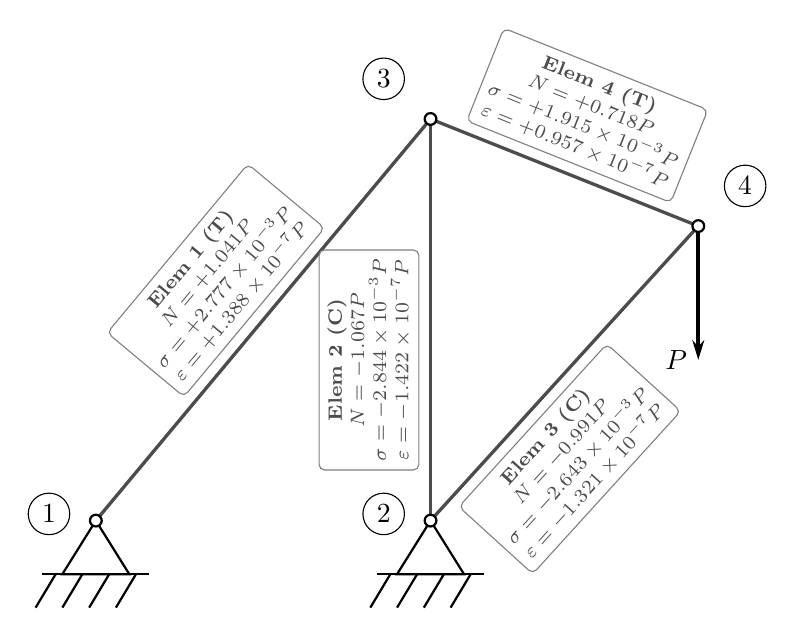
\begin{tikzpicture}[scale=1.7, >={Stealth[length=2.5mm, width=1.5mm]}]
        
        % --- Styles ---
        \tikzset{
            feLine/.style={very thick, black!70},
            feNode/.style={circle, draw=black, thick, fill=white, inner sep=1.5pt, minimum size=4pt},
            nodeLabel/.style={circle, draw, inner sep=1pt, minimum size=15pt},
            % Style for the results data box
            resultBox/.style={
                rectangle, draw=black!50, thin, fill=white, fill opacity=0.9, text opacity=1,
                align=center, font=\scriptsize, inner sep=3pt, rounded corners=2pt
            }
        }
        
        % --- Pinned Support Macro ---
        \def\drawPinSupport#1{
            \draw[thick] (#1) -- ++(-0.25, -0.4) -- ++(0.5, 0) -- cycle;
            \draw[thick] (#1) ++(-0.4, -0.4) -- ++(0.8, 0);
            \foreach \i in {-0.3, -0.1, 0.1, 0.3} {
                \draw[thick] (#1) ++(\i, -0.4) -- ++(-0.15, -0.25);
            }
        }

        % --- Coordinates ---
        \coordinate (N1) at (0,0);
        \coordinate (N2) at (2.5,0);
        \coordinate (N3) at (2.5,3.0);
        \coordinate (N4) at (4.5,2.2);
        
        % --- Draw Supports ---
        \drawPinSupport{N1}
        \drawPinSupport{N2}
        
        % --- Draw Elements with Result Boxes ---
        
        % Element 1 (1->3)
        \draw[feLine] (N1) -- (N3) node[midway, sloped, above=4pt, resultBox] {
            \textbf{Elem 1 (T)}\\
            $N = +1.041 P$\\
            $\sigma = +2.777 \times 10^{-3} P$\\
            $\varepsilon = +1.388 \times 10^{-7} P$
        };
        
        % Element 2 (2->3)
        \draw[feLine] (N2) -- (N3) node[pos=0.40, sloped, above=4pt, resultBox] {
            \textbf{Elem 2 (C)}\\
            $N = -1.067 P$\\
            $\sigma = -2.844 \times 10^{-3} P$\\
            $\varepsilon = -1.422 \times 10^{-7} P$
        };
        
        % Element 3 (2->4)
        \draw[feLine] (N2) -- (N4) node[pos=0.35, sloped, below=4pt, resultBox] {
            \textbf{Elem 3 (C)}\\
            $N = -0.991 P$\\
            $\sigma = -2.643 \times 10^{-3} P$\\
            $\varepsilon = -1.321 \times 10^{-7} P$
        };
        
        % Element 4 (3->4)
        \draw[feLine] (N3) -- (N4) node[midway, sloped, above=4pt, resultBox] {
            \textbf{Elem 4 (T)}\\
            $N = +0.718 P$\\
            $\sigma = +1.915 \times 10^{-3} P$\\
            $\varepsilon = +0.957 \times 10^{-7} P$
        };
        
        % --- Draw Applied Force P ---
        \draw[->, line width=1.5pt] (N4) -- ++(0,-1.0) node[pos=1, left]{$P$};
        
        % --- Draw Nodes (Top Layer) ---
        \node[feNode] at (N1) {};
        \node[feNode] at (N2) {};
        \node[feNode] at (N3) {};
        \node[feNode] at (N4) {};
        
        % --- Node Labels ---
        \node[nodeLabel] at ($(N1)+(-0.35, 0.05)$) {1};
        \node[nodeLabel] at ($(N2)+(-0.35, 0.05)$)  {2};
        \node[nodeLabel] at ($(N3)+(-0.35, 0.3)$)  {3};
        \node[nodeLabel] at ($(N4)+(0.35, 0.3)$)   {4};
        
    \end{tikzpicture}
    \caption{Internal normal forces, stresses, and strains for each element in terms of applied load $P$.}
    \label{fig:internal_results}
\end{figure}

% ======================================================================
\section{Part (d): First Yield}\label{sec:partd}
% ======================================================================

Yielding in element $e$ occurs when $|\sigma_e|=\sigma_y$, i.e.\ $P_y^{(e)}=\sigma_y\big/|\sigma_e/P|$:

\[
\begin{array}{c|c|c}
e & |\sigma_e/P|\;\text{(MPa/N)} & P_y^{(e)}\;\text{(N)} \\
\hline
1 & 2.777\times10^{-3} & 108\,031 \\
\mathbf{2} & \mathbf{2.844\times10^{-3}} & \mathbf{105\,469} \\
3 & 2.643\times10^{-3} & 113\,514 \\
4 & 1.915\times10^{-3} & 156\,680
\end{array}
\]

\begin{equation}\label{eq:yield}
\boxed{
\text{Element 2 yields first at } P_y = 105\,469 \text{ N} \approx 105.47 \text{ kN}\quad\text{(compression).}
}
\end{equation}

\noindent\textit{Verification at $P=105\,469$~N:}
\[
\begin{Bmatrix} \sigma_1 \\ \sigma_2 \\ \sigma_3 \\ \sigma_4 \end{Bmatrix}
= 105\,469 \times 10^{-3}\!
\begin{Bmatrix} +2.777 \\ -2.844 \\ -2.643 \\ +1.915 \end{Bmatrix}
=
\begin{Bmatrix} +292.9 \\ -300.0 \\ -278.7 \\ +201.9 \end{Bmatrix}
\text{\,MPa}
\quad\Longrightarrow\quad |\sigma_e| \le \sigma_y = 300\;\forall\, e
\]

% ======================================================================
\section{Part (e): First Buckling}\label{sec:parte}
% ======================================================================

Only compressed members ($N_e<0$) can buckle; from \cref{eq:strains}, these are elements 2 and 3.  For a pinned--pinned column, the Euler critical load is
\begin{equation}\label{eq:euler}
P_{\text{cr}}^{(e)} = \frac{\pi^2 E I}{L_e^2}.
\end{equation}

The section is a square hollow section with outer dimensions $40\times40$~mm and wall thickness $t=2.5$~mm.  Therefore
\[
A = 40^2-35^2 = 375\;\text{mm}^2,\qquad
I = \frac{40^4-35^4}{12} = 88\,281.25\;\text{mm}^4.
\]
The internal axial force in element $e$ is $|N_e|=|N_e/P|\times P$; buckling occurs when $|N_e|=P_{\text{cr}}^{(e)}$, i.e.
\[
P_{\text{buckle}}^{(e)} = \frac{P_{\text{cr}}^{(e)}}{|N_e/P|}.
\]

\[
\begin{array}{c|c|c|c|c}
e & L_e\;\text{(mm)} & |N_e/P| & P_{\text{cr}}^{(e)} = \dfrac{\pi^2 EI}{L_e^2}\;\text{(N)} & P_{\text{buckle}}^{(e)}=\dfrac{P_{\text{cr}}^{(e)}}{|N_e/P|}\;\text{(N)} \\[6pt]
\hline\rule{0pt}{14pt}
1 & 3905 & 1.041 & \text{---} & \text{tension, no buckling} \\
\mathbf{2} & \mathbf{3000} & \mathbf{1.067} & \dfrac{\pi^2\times20000\times88281.25}{3000^2} = \mathbf{1936.22} & \dfrac{1936.22}{1.067} = \mathbf{1815.21} \\[8pt]
3 & 2973 & 0.991 & \dfrac{\pi^2\times20000\times88281.25}{2973^2} = 1971.27 & \dfrac{1971.27}{0.991} = 1989.03 \\[8pt]
4 & 2154 & 0.718 & \text{---} & \text{tension, no buckling}
\end{array}
\]

\noindent Since $P_{\text{buckle}}^{(2)} < P_{\text{buckle}}^{(3)}$:

\begin{equation}\label{eq:buckle}
\boxed{
\text{Element 2 buckles first at } P_{\text{buckle}} = 1815.2 \text{ N} \approx 1.815 \text{ kN}\quad\text{(square hollow section).}
}
\end{equation}

\noindent\textit{Remark:}\; $P_{\text{buckle}}\approx1815$~N $\ll$ $P_y=105\,469$~N; buckling still governs.  The radius of gyration is $r=\sqrt{I/A}=15.34$~mm, so $\lambda_2=L_2/r=195.5$ and $\lambda_3=L_3/r=193.8$.

% ======================================================================
\section{Deformed Shape}
% ======================================================================

\begin{figure}[H]
\centering
    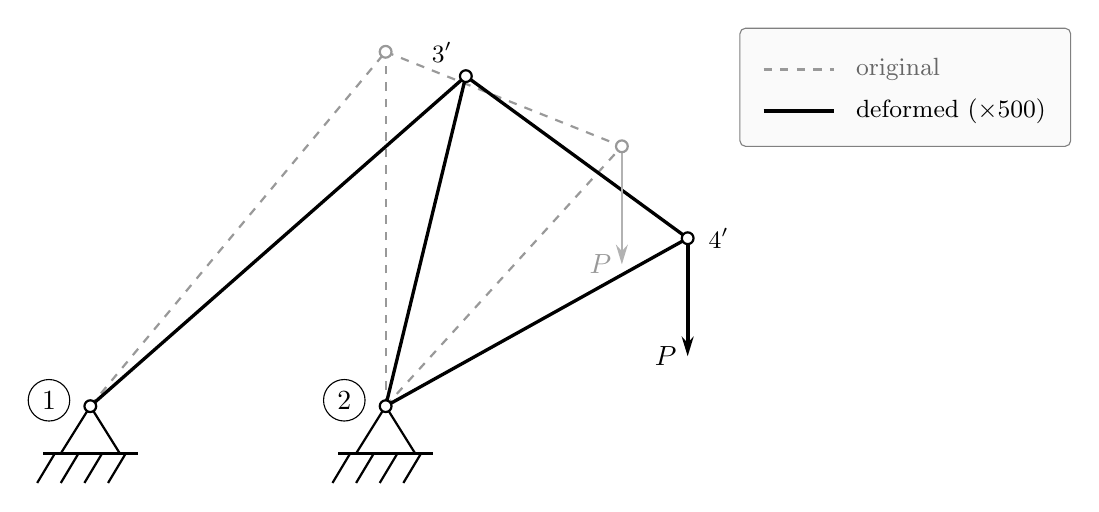
\begin{tikzpicture}[scale=1.5, >={Stealth[length=2.5mm, width=1.5mm]}]
        
        % --- Styles ---
        \tikzset{
            feLine/.style={very thick, black},
            origLine/.style={thick, dashed, black!40},
            feNode/.style={circle, draw=black, thick, fill=white, inner sep=1.5pt, minimum size=4pt},
            origNode/.style={circle, draw=black!40, thick, fill=white, inner sep=1.5pt, minimum size=4pt},
            nodeLabel/.style={circle, draw, inner sep=1pt, minimum size=15pt},
            legendBox/.style={draw=black!50, thin, fill=black!2, rounded corners=2pt}
        }
        
        % --- Pinned Support Macro ---
        \def\drawPinSupport#1{
            \draw[thick] (#1) -- ++(-0.25, -0.4) -- ++(0.5, 0) -- cycle;
            \draw[thick] (#1) ++(-0.4, -0.4) -- ++(0.8, 0);
            \foreach \i in {-0.3, -0.1, 0.1, 0.3} {
                \draw[thick] (#1) ++(\i, -0.4) -- ++(-0.15, -0.25);
            }
        }

        % --- Coordinates (Original) ---
        \coordinate (N1) at (0,0);
        \coordinate (N2) at (2.5,0);
        \coordinate (N3) at (2.5,3.0);
        \coordinate (N4) at (4.5,2.2);
        
        % --- Coordinates (Deformed - Scale Factor 500) ---
        \def\sf{500}
        \coordinate (D1) at (0,0);
        \coordinate (D2) at (2.5,0);
        \coordinate (D3) at ({2.5+1.359e-3*\sf},{3.0-4.267e-4*\sf});
        \coordinate (D4) at ({4.5+1.129e-3*\sf},{2.2-1.557e-3*\sf});
        
        % 1. Draw Supports (Bottom layer)
        \drawPinSupport{N1}
        \drawPinSupport{N2}
        
        % 2. Draw Lines (Original structure - Dashed)
        \draw[origLine] (N1)--(N3);
        \draw[origLine] (N2)--(N3);
        \draw[origLine] (N2)--(N4);
        \draw[origLine] (N3)--(N4);
        
        % 3. Draw Lines (Deformed structure - Solid)
        \draw[feLine] (D1)--(D3);
        \draw[feLine] (D2)--(D3);
        \draw[feLine] (D2)--(D4);
        \draw[feLine] (D3)--(D4);
        
        % 4. Draw Applied Forces P 
        % Faded force on original position
        \draw[->, line width=1pt, draw=black!30] (N4) -- ++(0,-1.0) node[pos=1, left, text=black!40]{$P$};
        % Solid force on deformed position
        \draw[->, line width=1.5pt] (D4) -- ++(0,-1.0) node[pos=1, left]{$P$};
        
        % 5. Draw Nodes (Top layer - covers lines beneath them)
        % Original nodes (only N3 and N4, as N1 and N2 don't move)
        \node[origNode] at (N3) {};
        \node[origNode] at (N4) {};
        
        % Deformed / Fixed nodes
        \node[feNode] at (D1) {};
        \node[feNode] at (D2) {};
        \node[feNode] at (D3) {};
        \node[feNode] at (D4) {};
        
        % 6. Labels
        \node[nodeLabel] at ($(N1)+(-0.35, 0.05)$) {1};
        \node[nodeLabel] at ($(N2)+(-0.35, 0.05)$)  {2};
        
        % Adjusted labels for displaced nodes to prevent overlap
        \node[above left=2pt, font=\small, text=black] at (D3) {$3'$};
        \node[right=4pt, font=\small, text=black] at (D4) {$4'$};
        
        % 7. Legend (Framed box, perfectly aligned)
        \begin{scope}[shift={(5.5, 3.2)}]
            \draw[legendBox] (0, 0) rectangle (2.8, -1.0);
            
            \draw[origLine] (0.2, -0.35) -- (0.8, -0.35);
            \node[right, font=\small, text=black!60] at (0.9, -0.35) {original};
            
            \draw[feLine] (0.2, -0.7) -- (0.8, -0.7);
            \node[right, font=\small] at (0.9, -0.7) {deformed ($\times500$)};
        \end{scope}
        
    \end{tikzpicture}
\caption{Original (dashed) and exaggerated deformed shape.}
\label{fig:deformed}
\end{figure}



% ======================================================================
\section{OpenSees Validation}
% ======================================================================

The hand-computation results are independently validated using \textbf{OpenSeesPy~3.5.1} (run in a \texttt{conda} environment with Python~3.10).  The same truss is modelled with \texttt{Truss} elements and an \texttt{Elastic} material ($E=20\,000$~MPa, $A=375$~mm$^2$).  The hollow-section moment of inertia $I=88\,281.25$~mm$^4$ is then used in the Euler buckling post-processing step.

\medskip
\noindent\textbf{Displacement comparison} (per unit $P=1$~N):

\[
\begin{array}{c|cc|cc|c}
\text{Node} & u_{\text{hand}} & u_{\text{OS}} & v_{\text{hand}} & v_{\text{OS}} & \text{Max.\ rel.\ err.} \\
\hline
3 & +1.35898\!\times\!10^{-3} & +1.35898\!\times\!10^{-3} & -4.26667\!\times\!10^{-4} & -4.26667\!\times\!10^{-4} & $<0.001\%$ \\
4 & +1.12887\!\times\!10^{-3} & +1.12887\!\times\!10^{-3} & -1.55722\!\times\!10^{-3} & -1.55722\!\times\!10^{-3} & $<0.001\%$
\end{array}
\]

\noindent\textbf{Strain and force comparison}:

\[
\begin{array}{c|cc|c}
e & \varepsilon_{\text{hand}}/P & \varepsilon_{\text{OS}}/P & \text{Rel.\ err.} \\
\hline
1 & +1.38849\!\times\!10^{-7} & +1.38849\!\times\!10^{-7} & $<0.001\%$ \\
2 & -1.42222\!\times\!10^{-7} & -1.42222\!\times\!10^{-7} & $<0.001\%$ \\
3 & -1.32143\!\times\!10^{-7} & -1.32143\!\times\!10^{-7} & $<0.001\%$ \\
4 & +9.57363\!\times\!10^{-8} & +9.57363\!\times\!10^{-8} & $<0.001\%$
\end{array}
\]

\noindent\textbf{Critical loads}:

\[
\begin{array}{l|cc}
 & \text{Hand} & \text{OpenSees} \\
\hline
\text{First yield (Elem.\ 2)} & P_y = 105\,468.75\;\text{N} & P_y = 105\,468.750\;\text{N} \\
\text{First buckling (Elem.\ 2)} & P_{\text{cr}} = 1815.21\;\text{N} & P_{\text{cr}} = 1815.210\;\text{N}
\end{array}
\]

\noindent All results match to within rounding, confirming the hand computation.  The support reactions also satisfy equilibrium exactly: $\sum F_x = 0$, $\sum F_y = 0$, $\sum M = 0$.
% ======================================================================
\section{Discussion}
% ======================================================================

\subsection{Demand vs.\ Capacity}

The analysis reveals a \textbf{critical imbalance} between the two failure modes:
%
\[
\frac{P_y}{P_{\text{cr}}} = \frac{105\,469}{1815.2} \approx 58.1.
\]
%
The Euler buckling load of Element~2 ($P_{\text{cr}}=1815.2$~N) is still about \textbf{58 times smaller} than the yield load ($P_y=105\,469$~N).  The new hollow section improves stiffness and buckling resistance significantly, but the structure still fails by buckling well before any material yielding occurs.  Material capacity therefore remains underutilised.

\subsection{Role of Each Element}

\begin{table}[H]
\centering
\small
\renewcommand{\arraystretch}{1.25}
\begin{tabular}{@{}clccccl@{}}
\toprule
$e$ & Connectivity & $L$ (mm) & $\sigma_e$ at $P_y$ & Nature & $\lambda$ & Assessment \\
\midrule
1 & $1{\to}3$ (diagonal) & 3905.1 & $+292.9$ & T & 254.5 & Near yield; efficiently utilised. \\
  &                       &        &          &   &       & Buckling not relevant (tension). \\[3pt]
2 & $2{\to}3$ (vertical) & 3000.0 & $-300.0$ & C & 195.5 & \textbf{Critical element.} Yields first \\
  &                       &        &          &   &       & \emph{and} buckles first ($P_{\text{cr}}^{(2)}=1936.2$~N). \\[3pt]
3 & $2{\to}4$ (diagonal) & 2973.2 & $-278.7$ & C & 193.8 & Buckles shortly after Elem.~2 \\
  &                       &        &          &   &       & ($P_{\text{cr}}^{(3)}=1971.3$~N). \\[3pt]
4 & $3{\to}4$ (upper)    & 2154.1 & $+201.9$ & T & 140.4 & Well below yield; no buckling risk. \\
\bottomrule
\end{tabular}
\caption{Element summary at $P_y=105\,469$~N.  T = tension, C = compression.  $\lambda = L/r$, \, $r = \sqrt{I/A}=15.34$~mm.}
\label{tab:elem_roles}
\end{table}

\subsection{Design Deficiencies and Recommendations}

\begin{table}[H]
\centering
\small
\renewcommand{\arraystretch}{1.3}
\begin{tabular}{@{}cp{5.5cm}p{5.5cm}@{}}
\toprule
\# & Deficiency & Recommendation \\
\midrule
1 & \textbf{Buckling capacity remains low.}  Elements~2 and 3 have $\lambda\approx195$, and the governing external buckling load is only $1.82$~kN.
  & Increase member inertia or reduce effective length.  Matching $P_{\text{cr}}$ to $P_y$ requires about $58$ times the current Euler capacity. \\
\midrule
2 & \textbf{Buckling governs.} $P_y/P_{\text{cr}}\approx58$; material capacity is still wasted.
  & Balance stability and strength such that $P_{\text{cr}} \gtrsim P_y$. \\
\midrule
3 & \textbf{No lateral bracing.}  Effective buckling lengths equal full member lengths.
  & Add mid-span braces to Elem.~2 and 3; halving $L_{\text{eff}}$ quadruples $P_{\text{cr}}$ to about $7.26$~kN, still below $P_y$ but safer than the unbraced case. \\
\midrule
4 & \textbf{No redundancy.}  Statically determinate: loss of any element $\Rightarrow$ collapse.
  & Add diagonal brace $1{\to}4$ for alternative load path and robustness. \\
\bottomrule
\end{tabular}
\caption{Design deficiencies and engineering recommendations.}
\label{tab:recommendations}
\end{table}

\subsection{Demand/Capacity Summary}

At the first buckling load $P = 1815.2$~N:

\begin{table}[H]
\centering
\small
\renewcommand{\arraystretch}{1.2}
\begin{tabular}{@{}crrcrl@{}}
\toprule
$e$ & $\sigma_e$ (MPa) & $\sigma_e / \sigma_y$ & D/C (yield) & $P_{\text{cr}}^{(e)}$ (N) & D/C (buckle) \\
\midrule
1 & $+5.041$ & 0.017 & OK & --- & tension \\
2 & $-5.163$ & 0.017 & OK & 1936.2 & $\mathbf{1.00}$ \\
3 & $-4.797$ & 0.016 & OK & 1971.3 & 0.91 \\
4 & $+3.476$ & 0.012 & OK & --- & tension \\
\bottomrule
\end{tabular}
\caption{Demand/capacity ratios at $P=1815.2$~N (first buckling).}
\label{tab:dc_ratios}
\end{table}

\noindent Element~2 reaches D/C $= 1.0$ for buckling while all yield D/C ratios remain small ($\le 1.7\%$).  This confirms that \textbf{stability, not strength, is the governing limit state}, and the design must still be revised to raise the buckling capacity of the compression members.

% ======================================================================
\section{Conclusion}
% ======================================================================

The key findings are summarised below.

\begin{table}[H]
\centering
\small
\renewcommand{\arraystretch}{1.25}
\begin{tabular}{@{}lp{10cm}@{}}
\toprule
\textbf{Aspect} & \textbf{Finding} \\
\midrule
Assembly &
The $8\!\times\!8$ global stiffness matrix was assembled from four element contributions using the direct stiffness method.  After applying the boundary conditions ($u_1=v_1=u_2=v_2=0$), the reduced $4\!\times\!4$ system was solved for the free DOFs at Nodes~3 and 4. \\[3pt]
Displacement &
The free-node displacements scale linearly with $P$.  Node~4 undergoes the largest vertical displacement ($v_4 = -1.557\!\times\!10^{-3}\,P$~mm), consistent with the load application point. \\[3pt]
Internal forces &
Elements~1 and 4 carry tension; Elements~2 and 3 carry compression.  Element~2 carries the largest compressive force ($N_2 = -1.067\,P$~N), making it the most critical member. \\[3pt]
First yield &
First yielding occurs in Element~2 at $P_y = 105\,469$~N ($\sigma_2 = -\sigma_y = -300$~MPa). \\[3pt]
First buckling &
Euler buckling of Element~2 occurs at $P_{\text{cr}} = 1815.2$~N, which is still \textbf{58.1 times lower} than the yield load.  Stability, not material strength, governs the design. \\[3pt]
Validation &
Independent analysis using OpenSeesPy~3.5.1 confirms the updated hand-computation results to within rounding.  Equilibrium of reactions is exactly satisfied. \\[3pt]
Design &
The current $40\!\times\!40\!\times\!2.5$~mm square hollow section reduces slenderness to about $\lambda\approx195$, but the compression members still buckle far before yielding.  A larger section and/or shorter effective buckling length is required. \\
\bottomrule
\end{tabular}
\caption{Summary of key findings.}
\label{tab:conclusion}
\end{table}

\noindent In conclusion, the direct stiffness method provides an exact linear elastic solution for this truss system.  The revised hollow-section model shows that the structure has substantial material capacity ($P_y = 105.47$~kN), yet it is still rendered structurally inadequate by premature Euler buckling at $P_{\text{cr}} = 1.815$~kN.  A practical redesign must therefore increase compression-member stability, not merely material strength, before the structure can be deployed safely.

\end{document}
